\chapter{Methods}
% Methods
\section{Methods}
Other publications that consider \ac{CoM} height variations for balance use \ac{MPC}. Considering worst-case scenario's, where additional horizontal force is needed, `the best you can do' is needed to not fall over. This motivates to use a proportional controller in worst case scenario's, next to the benefit of simplicity and robustness.

%Challenges
\subsection{Challenges}
\subsubsection{Angular Momentum} has a lot
\subsubsection{2D to 3D}
\subsubsection{Leg Reachability}
\subsubsection{Predictability of Dynamics}

%Architecture
\subsection{Control Framework}
To actively change the desired momentum rate, the effects of additional height acceleration is included in the control framework as follows. 
Horizontal linear momentum rate formula in terms of \ac{CMP}:
\begin{equation}
\dot{\mathbf{l}}_{xy}=\frac{\mathbf{c}_{xy}-\mathbf{r}_{cmp}}{z}F_z
\end{equation}
Horizontal linear momentum rate formula in terms of \ac{CoP}:
\begin{equation}
\dot{\mathbf{l}}_{xy}=\frac{\mathbf{c}_{xy}-(\mathbf{r}_{cop}+\frac{\tau_y}{F_z})}{z}F_z
\end{equation}
\begin{equation}
\dot{\mathbf{l}}_{xy}=\frac{\mathbf{c}_{xy}-\mathbf{r}_{cop}}{z}m(g+\ddot{z}) - \frac{\tau_y}{z}
\end{equation}
\begin{equation}
\dot{\mathbf{l}}_{xy}=\frac{\mathbf{c}_{xy}-\mathbf{r}_{cop}}{z}mg - \frac{\tau_y}{z} + \frac{\mathbf{c}_{xy}-\mathbf{r}_{cop}}{z}m\ddot{z}
\end{equation}
 Since the desired \ac{CMP} coming from the linear momentum rate of change control module is based on the \ac{LIP} model:
 \begin{equation}
\dot{\mathbf{l}}_{xy,d}=\underbrace{ \frac{\mathbf{c}_{xy}-\mathbf{r}_{cmp,d}} {z_0}mg}_{\dotldxylip}  + \underbrace{\frac{\mathbf{c}_{xy}-\mathbf{r}_{cop,d}}{z}m\ddot{z}_d}_{\dotldxyheight},
\end{equation}
where $\dotldxylip$ is the standard desired horizontal momentum rate term and $\dotldxyheight$ is the additional momentum rate from height control.
\subsubsection{Condition to Activate Controller}
In the control framework, $\rcmpd$ is restricted to be within a certain distance from the support polygon. During normal walking, the mentioned control framework is not activated, as $\rcmpd$ stays within the polygon, as with human walking [REF]. When the desired \ac{CMP} is farther away than a fraction of the maximum distance $\delta_{\rcmpd-polygon}>\fraccmp\delta_{\rcmpd-polygon,max}$, the height controller is activated for the remaining time in the swing phase. The default height trajectory is neglected and $\dotldxy$ is affected by the vertical acceleration.

%Strategy 
\subsection{Control Strategy}
With the control law to modify the existing $\dotldxylip$ with $\dotldxyheight$, the question remains how to generate the desired height acceleration $\ddzd$. A control strategy is considered for a worst case scenario, where height control can give that extra bit of balance. For situations where height variations are considered that are not worst-case, it is assumed that difference in height from the \ac{LIP} can be controlled using the allowed ``ankle'' and ``hip'' strategies. Therefore consider a `best doable' strategy . If an optimization outputs com(t), its is hard to include angular momentum, and still it's PD-controlled. 
$\rcmpd$ is restricted to remain a certain distance from the foot polygon. If $\rcmpd$ is over a fraction $\fraccmp$ from the maximum allowed distance outside the foot polygon, the height controller kicks in. As the robot in this case almost falls over, it is important to do the best it can to recover. Therefore, a maximum or minimum acceleration is considered, depending on the current condition. The controller is only allowed to opperate in \ac{SS}. In \ac{DS} is observed that it can cause problems with lift-off of the upcoming swing leg. The default height controller tries to bring the \ac{CoM} back to the height defined by the trajectory.  

%
\subsubsection{Alignment}


\subsubsection{Constraints}
The maximum length of the leg describes a part of a circle throught the swing phase. In the controller, this constraint is captured in two constraints: $\zmaxfirst$, in the first halve of the swing phase and $\zmaxscnd$, in the second part of the swing phase. In \figref{fig:heightconstraints} the two constraints are vizualized. 
\begin{figure}[h]
\centering
  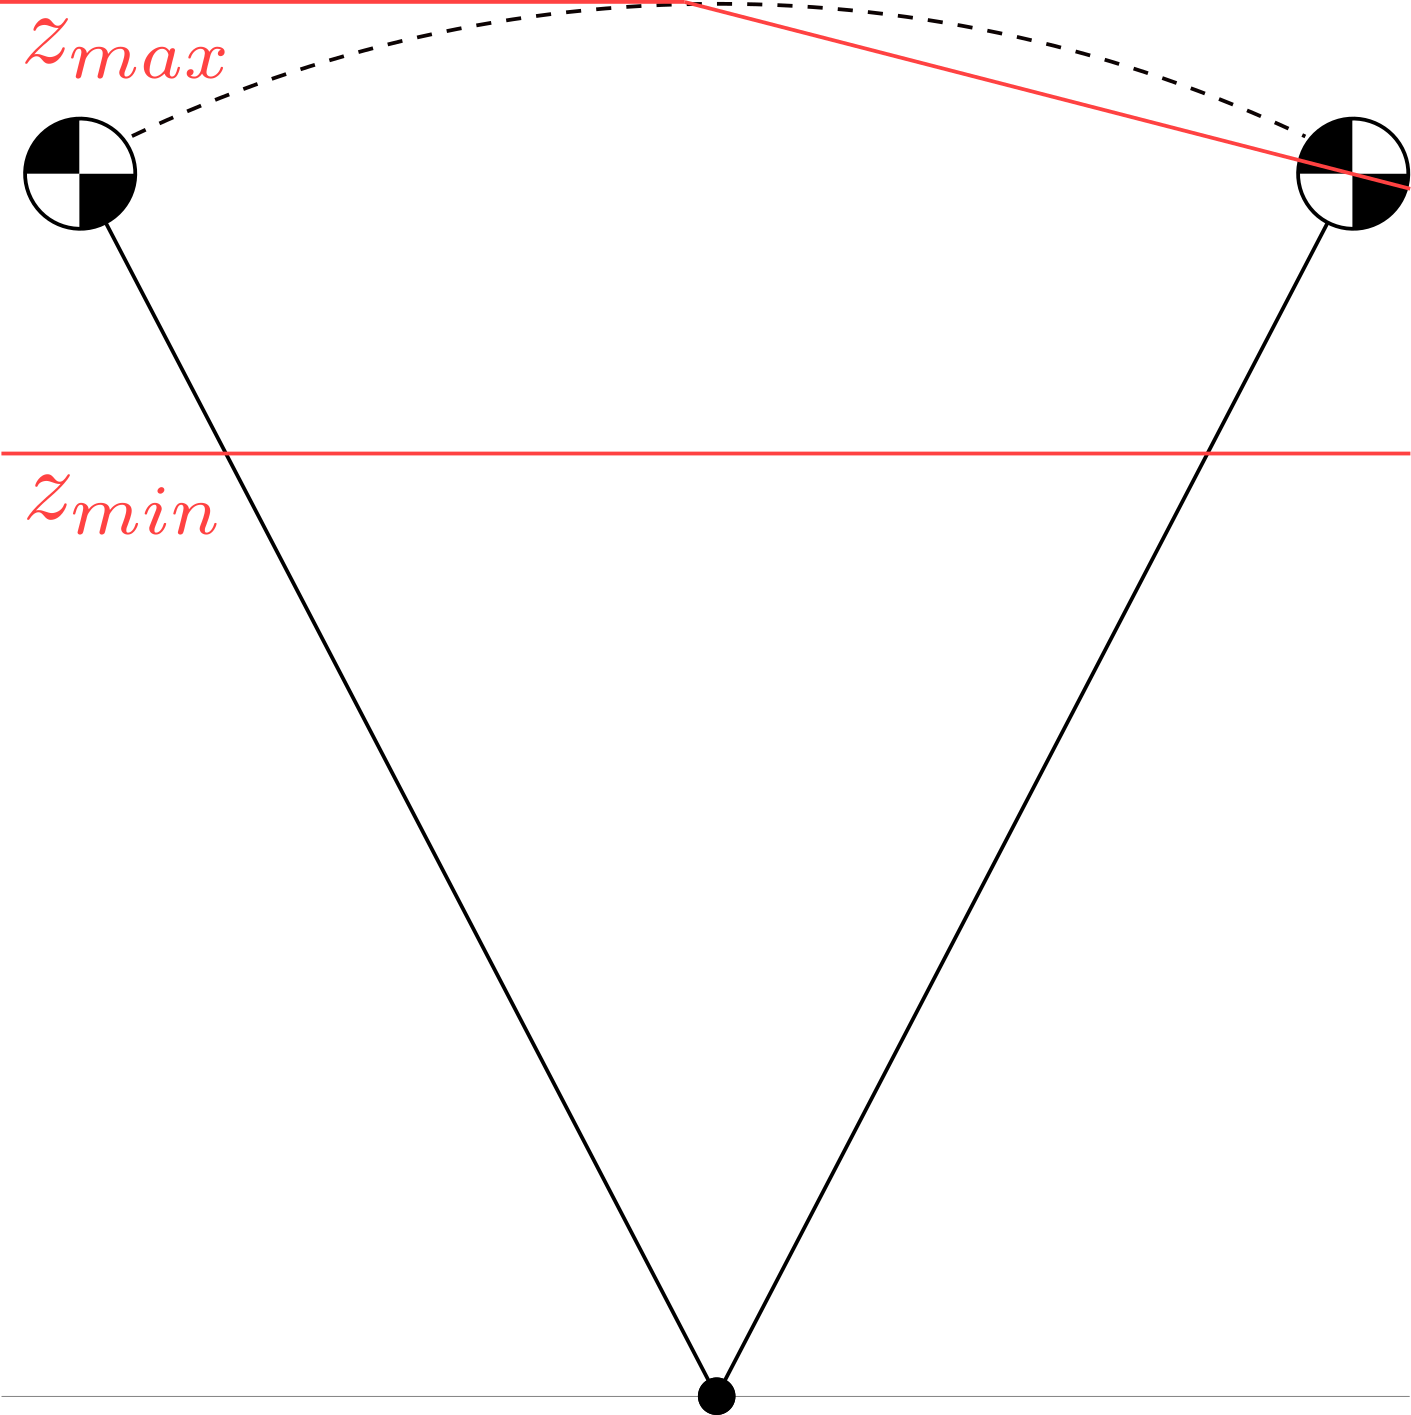
\includegraphics[width=.4\linewidth]{STYLESTUFF/heightconstraints.png}
   \caption{Height constraints through \ac{SS}}
    \label{fig:heightconstraints}
\end{figure} 
The predicted height the current state is about to reach is computed as:
\begin{equation}
	\zmaxpred = z + \sgn(\dot{z})\frac{\dot{z}^2}{-2\ddzminpred},
\end{equation}
where $\zmaxpred$ is the predicted maximum height from the current state and $\ddzminpred$ is the predicted maximum deceleration that will occur. This would be the gravity acceleration, but the minimal acceleration is limited. 
\paraskip
The minimum height constraint is not dependent on singularity of the swing leg and is kept at a constant value. Next to hitting the ground, a low height can cause problems at transfer to \ac{DS}, when the robot gets raised to default height again. The minimum height constraint $\zmin$ is displayed in \figref{fig:heightconstraints}. In a similar way as $\zmaxpred$, the minimum height constraint is computed as:
\begin{equation}
	\zminpred = z - \sgn(\dot{z})\frac{\dot{z}^2}{2\ddzmaxpred},
\end{equation}
where $\zminpred$ is the predicted minimum height from the current state and $\ddzmaxpred$ is the predicted maximum acceleration that will occur.
\paraskip
Contraints on the maximum height velocity $\dzmax$ and minimum height velocity $\dzmin$ are also taken into account. Reasons for this include collapsing of the swing leg at touch down and limited velocities at the robot. 


\subsubsection{Time Prediction To Constraints}
Time to maximum constraint, considered the minimum and maximum acceleration:
\begin{equation}
    z + \dot{z}\tzmax + \frac{1}{2}\ddzdmax\tzmax^2 + \frac{1}{2}\frac{(\dot{z} +\ddzdmax\tzmax)^2}{-\ddzminpred}= \zmax,
\end{equation}
where $\tzmax$ can be computed in the following way:
\begin{equation}
    \underbrace{\frac{1}{2}(\ddzdmax + \frac{\ddzdmax^2}{-\ddzminpred})}_a\tzmax^2 + \underbrace{(\dot{z} + \dot{z}\frac{\ddzdmax}{-\ddzminpred})}_b\tzmax + \underbrace{z - \zmax + \frac{1}{2}\frac{\dot{z}^2}{-\ddzminpred}}_c.
\end{equation}
Noting that $a$ is positive and that the time needs to be the positive solution, the predicted time to the maximum constraint reads as:
\begin{equation}
    \tzmax=\frac{-b + \sqrt{b^2 -4ac}}{2a}
\end{equation}
\paraskip
The predicted time to the minimum constraint is computed in a similar way:
\begin{equation}
    z + \dot{z}\tzmin + \frac{1}{2}\ddzdmin\tzmin^2 - \frac{1}{2}\frac{(\dot{z} +\ddzdmin\tzmin)^2}{\ddzmaxpred}= \zmin,
\end{equation}
where $\tzmin$ is computed as:
\begin{equation}
    \underbrace{\frac{1}{2}(\ddzdmin - \frac{\ddzdmin^2}{\ddzmaxpred})}_a\tzmin^2 + \underbrace{(\dot{z} - \dot{z}\frac{\ddzdmin}{\ddzmaxpred})}_b\tzmin + \underbrace{z - \zmax + \frac{1}{2}\frac{\dot{z}^2}{\ddzmaxpred}}_c.
\end{equation}
Noting that $a$ is strictly negative and that the time needs to be the positive solution, the predicted time to the minimum height constraint reads as:
\begin{equation}
    \tzmin=\frac{-b - \sqrt{b^2 -4ac}}{2a}
\end{equation}
\paraskip
The time to the maximum and mimimum velocity can be computed using a linear equation:
\begin{equation}
	\tdzmax = \frac{\dzmax - \dot{z}}{\ddzdmax}
\end{equation}
\begin{equation}
	\tdzmin = \frac{\dzmin - \dot{z}}{\ddzdmin}
\end{equation}

\subsubsection{Control Law}
Constraints have to be avoided in computation of input.\\


\begin{figure}[h]
\centering
  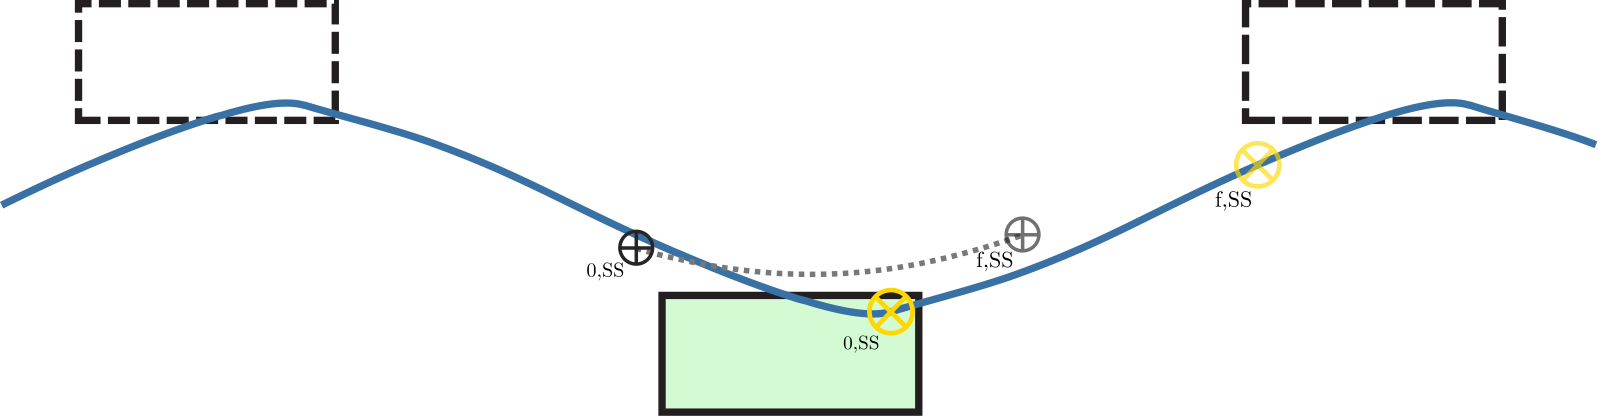
\includegraphics[width=.8\linewidth]{STYLESTUFF/ICPplan3StepComICPrSS.png}
   \caption{Initial (0,SS) and final (f,SS) configurations of \ac{CoM} position (black circle with cross) and \ac{ICP} reference (yellow circle with rotated cross) for \ac{SS} in the $xy$-plane with the parameters from Table \tabref{tab:stepping}. The green area is the current supporting foothold and the blue line is the \ac{ICP} reference trajectory.}
    \label{fig:3foot}
\end{figure}


\begin{figure}[h]
  \begin{subfigure}{0.5\textwidth}
  \centering
  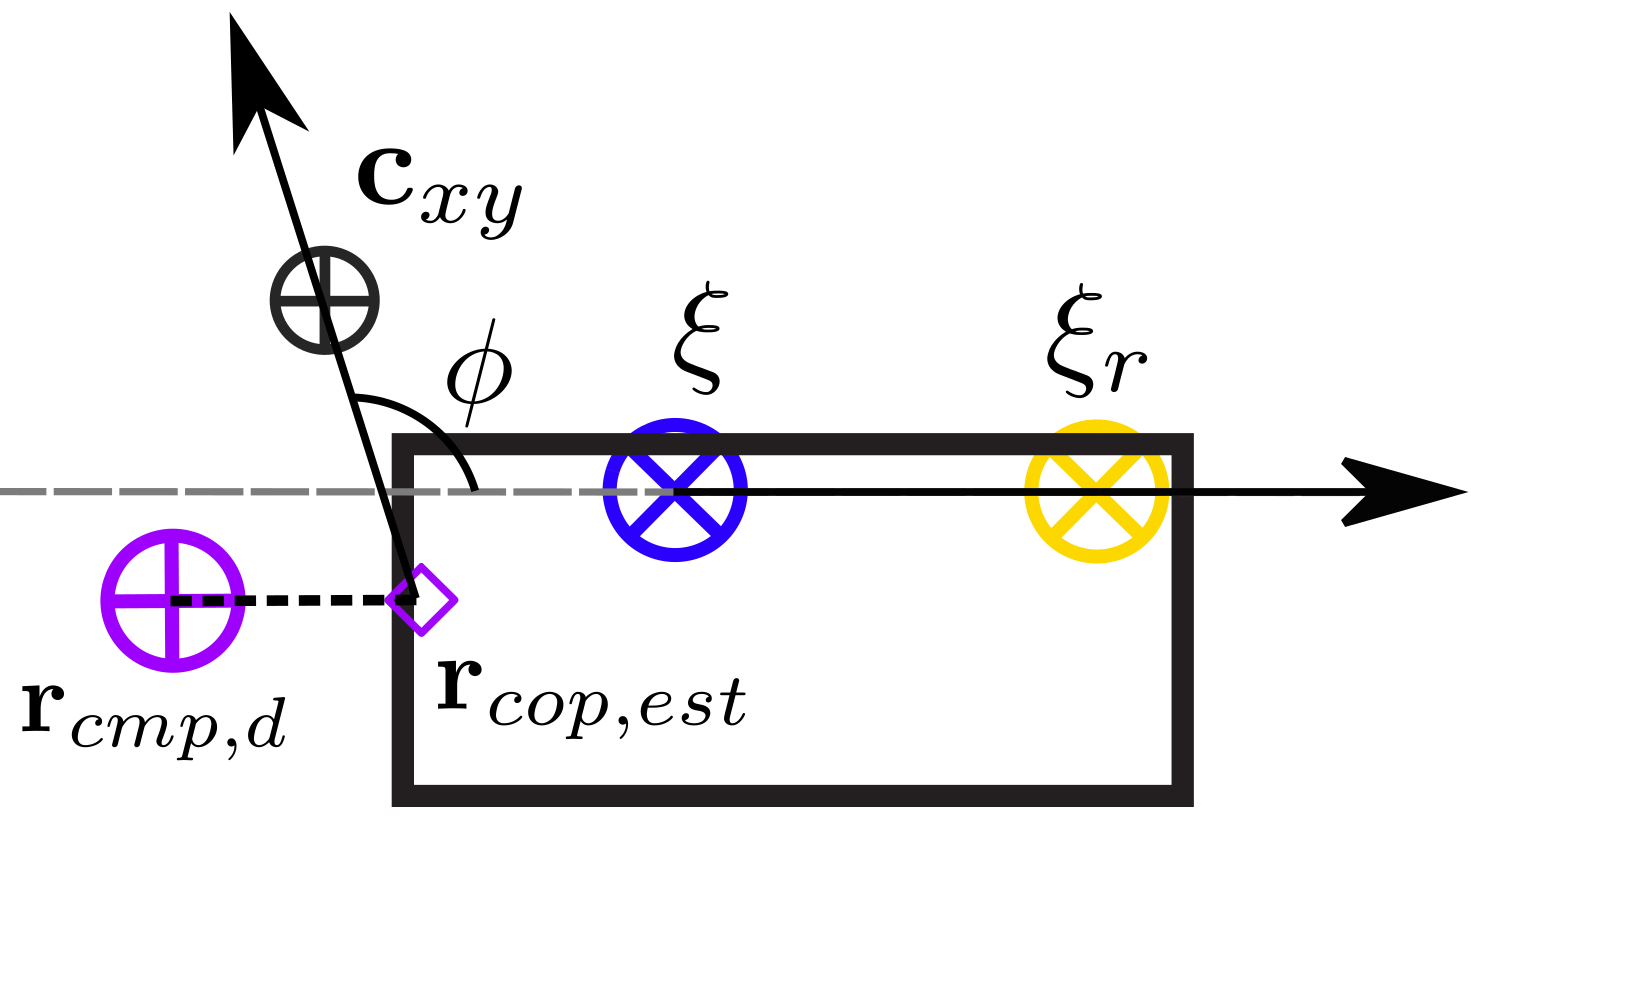
\includegraphics[width=.8\linewidth]{STYLESTUFF/ICPplanStartSSPhiViz.png}
   \caption{}
    \label{fig:phiViza}
  \end{subfigure}
  \begin{subfigure}{0.5\textwidth}
    \centering
  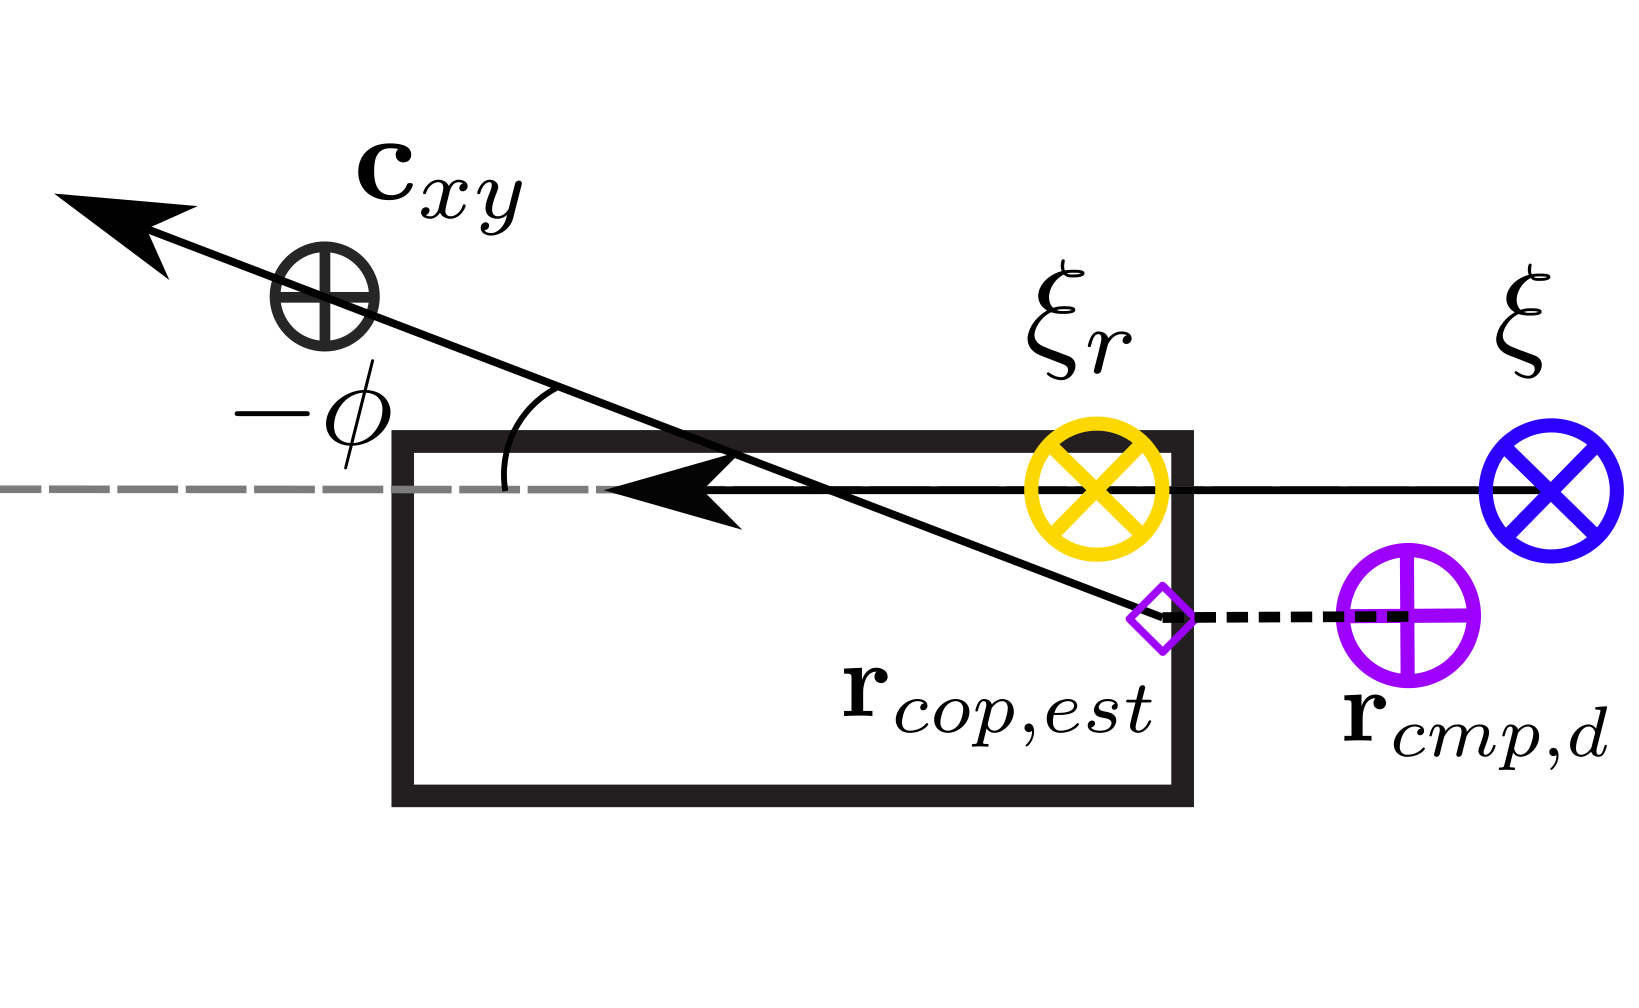
\includegraphics[width=.8\linewidth]{STYLESTUFF/ICPplanStartSSPhiVizNegError.png}
  \caption{}
   \label{fig:phiVizb}
  \end{subfigure}
  \begin{subfigure}{0.5\textwidth}
    \centering
  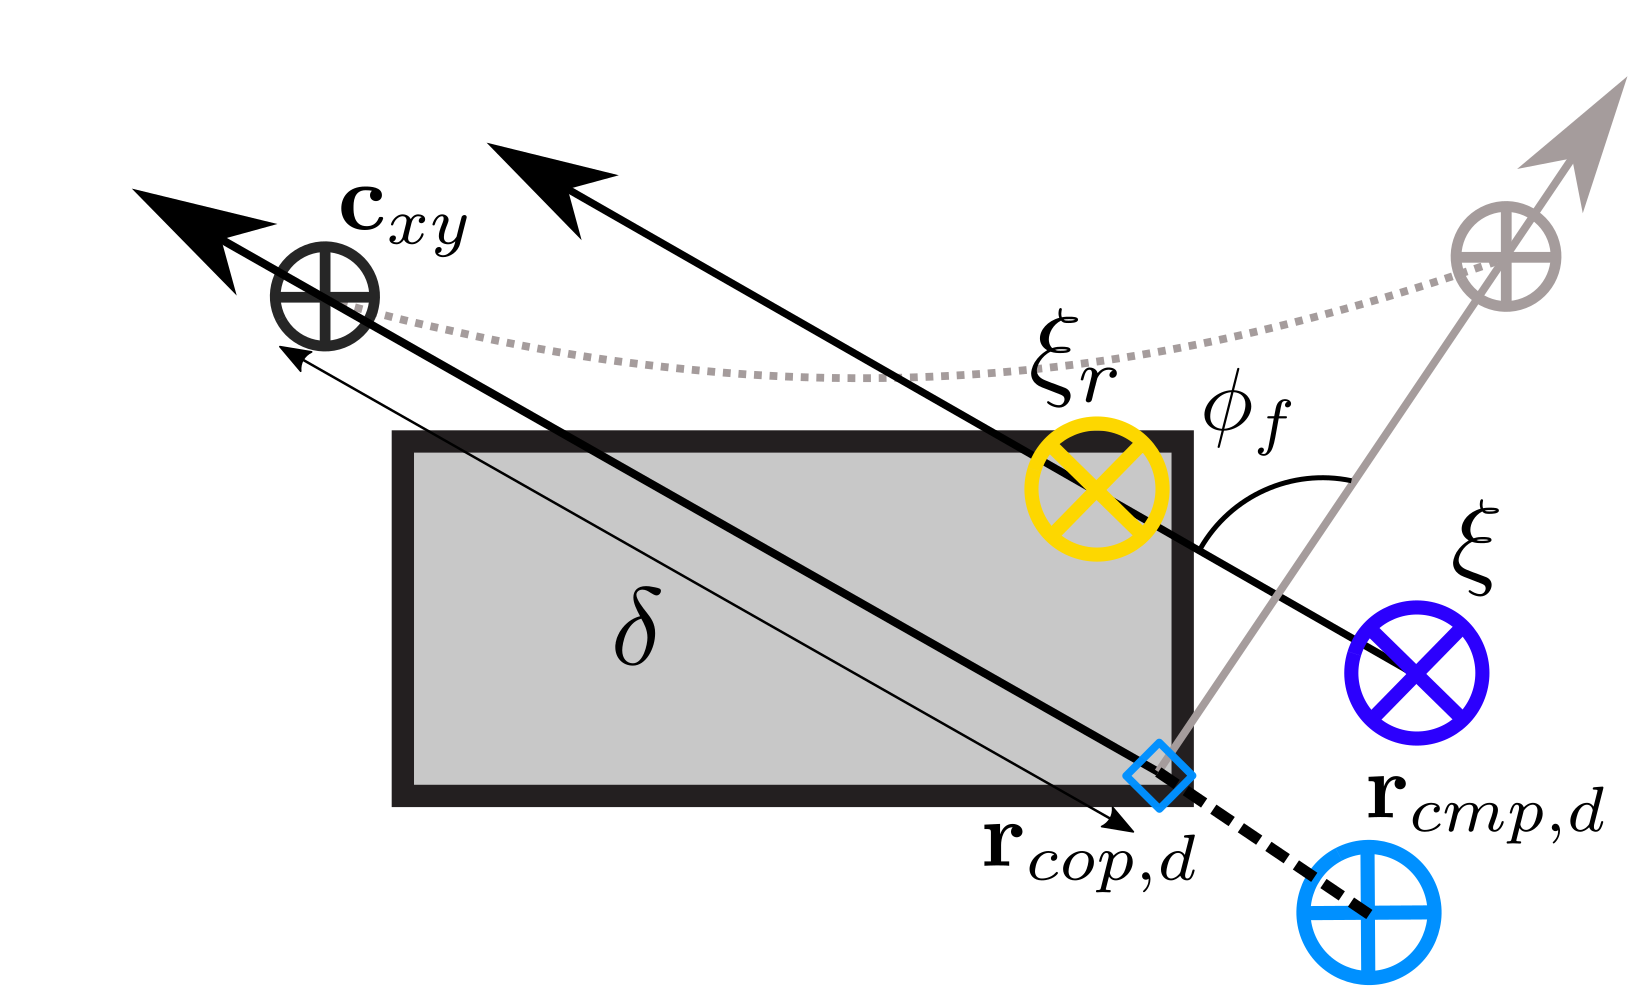
\includegraphics[width=.8\linewidth]{STYLESTUFF/ICPplanStartSSPhiViz0.png}
    \caption{}
     \label{fig:phiVizc}
  \end{subfigure}
  \begin{subfigure}{0.5\textwidth}
    \centering
  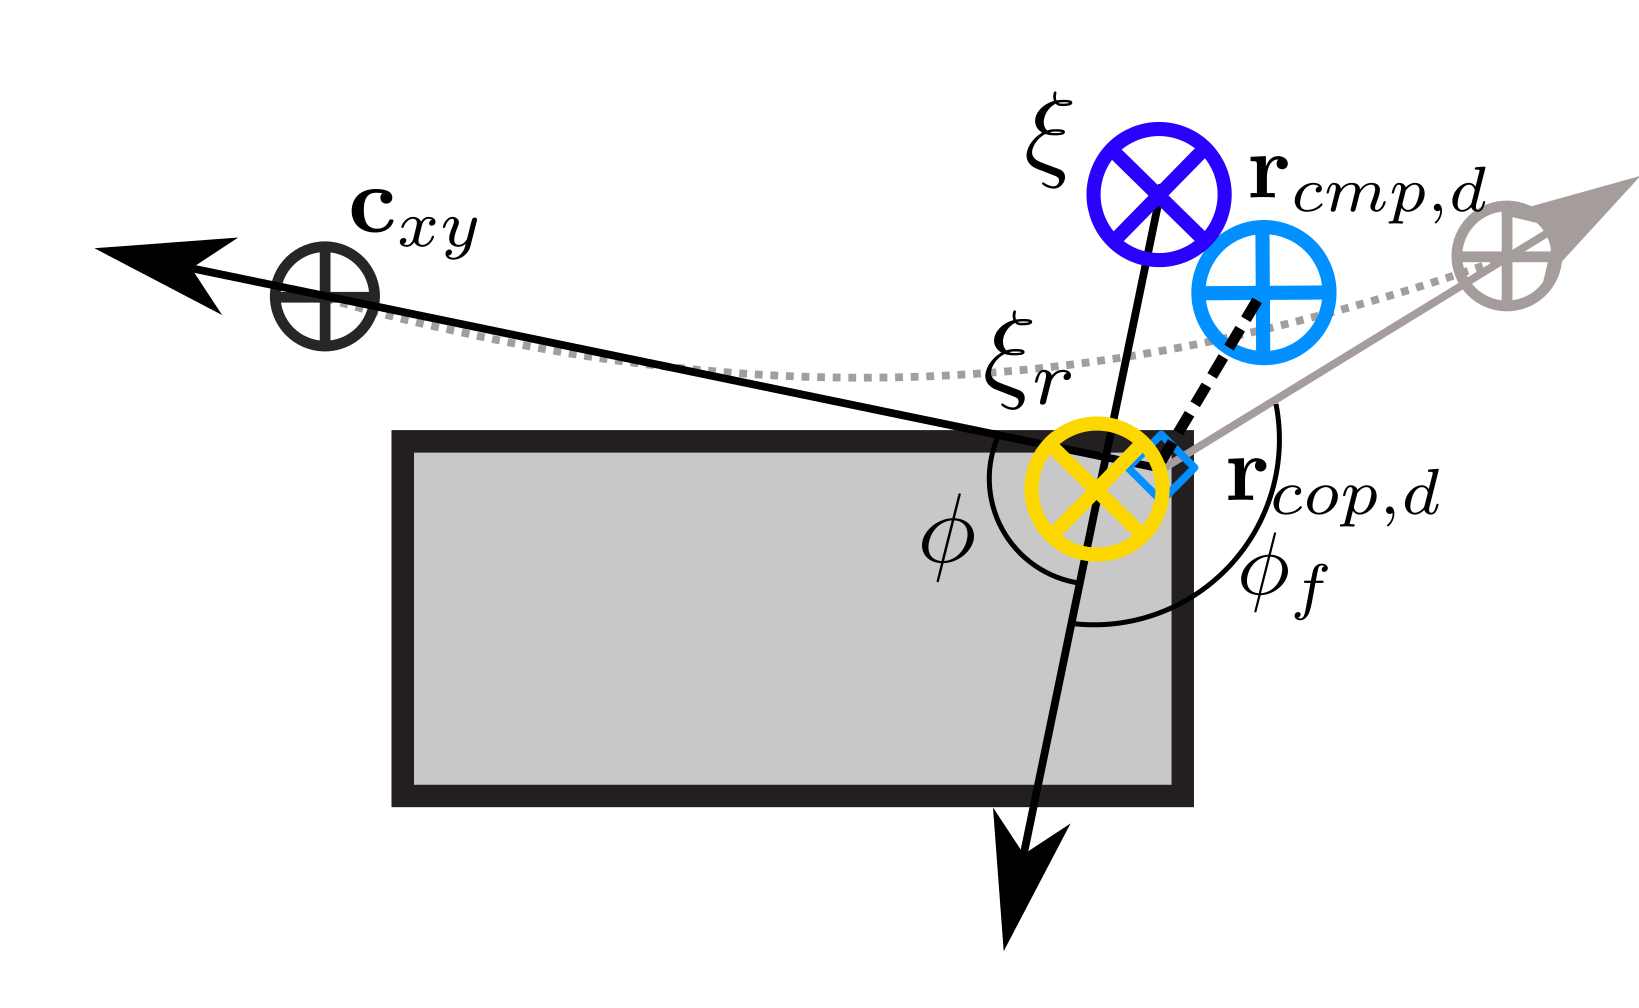
\includegraphics[width=.8\linewidth]{STYLESTUFF/ICPplanStartSSPhiViz90.png}
    \caption{}
     \label{fig:phiVizd}
  \end{subfigure}
    \begin{subfigure}{0.5\textwidth}
    \centering
  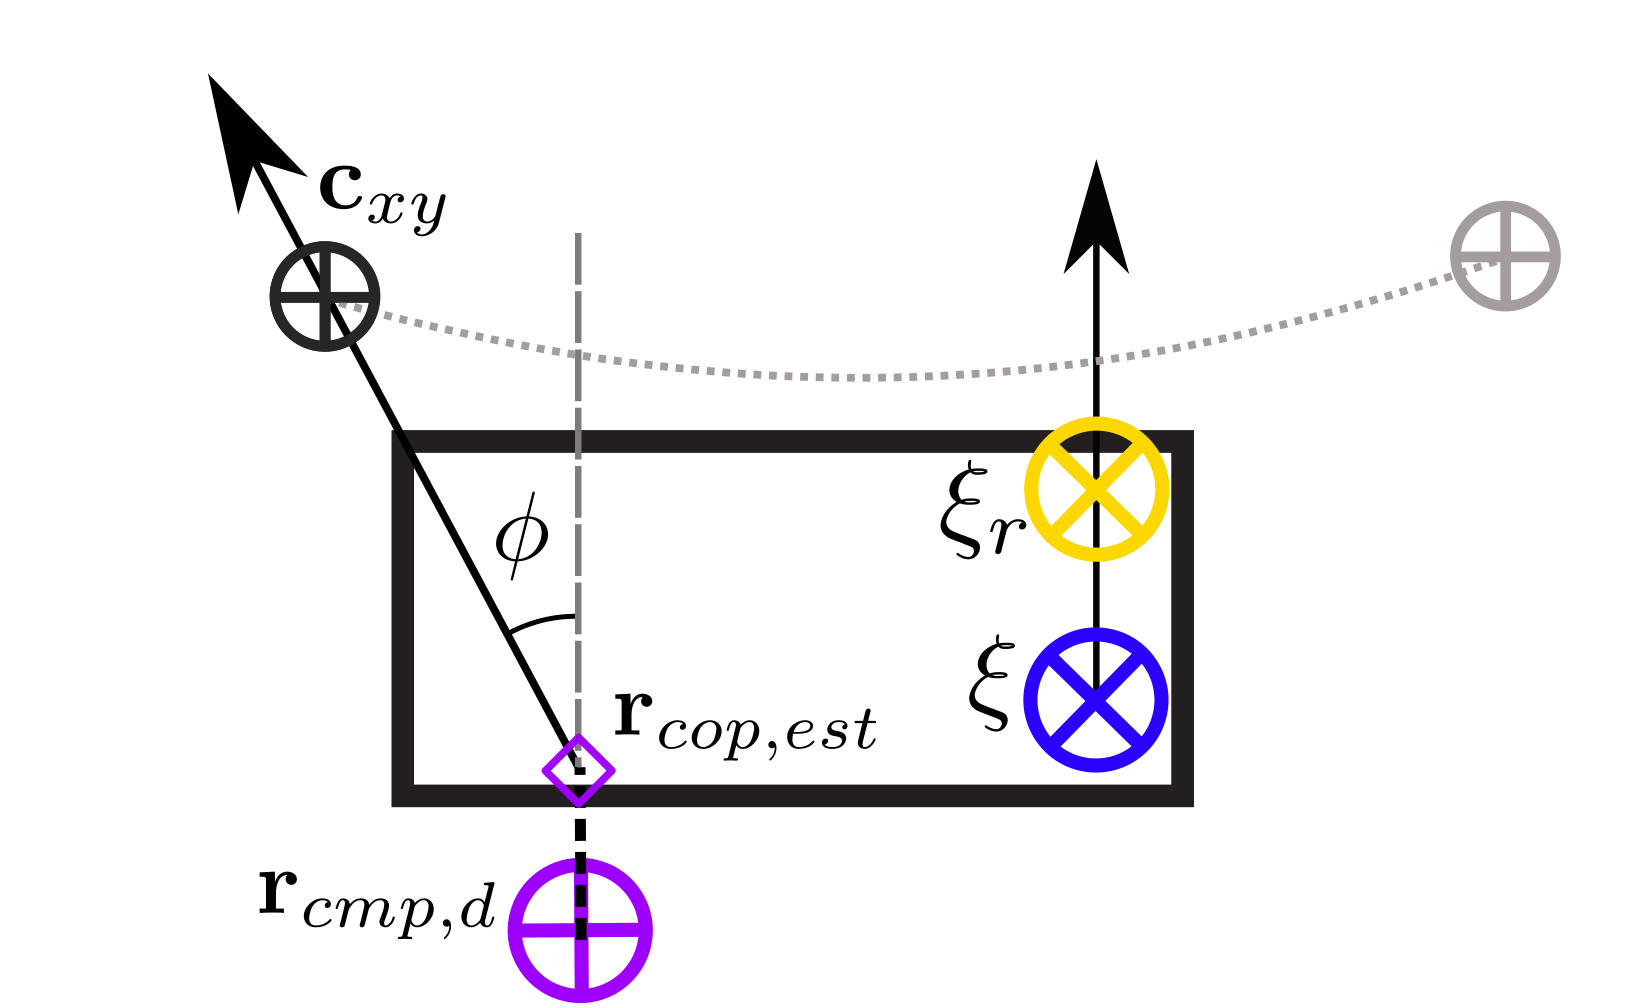
\includegraphics[width=.8\linewidth]{STYLESTUFF/ICPplanStartSSPhiVizLeftError.png}
    \caption{}
     \label{fig:phiVize}
  \end{subfigure}
  \begin{subfigure}{0.5\textwidth}
    \centering
  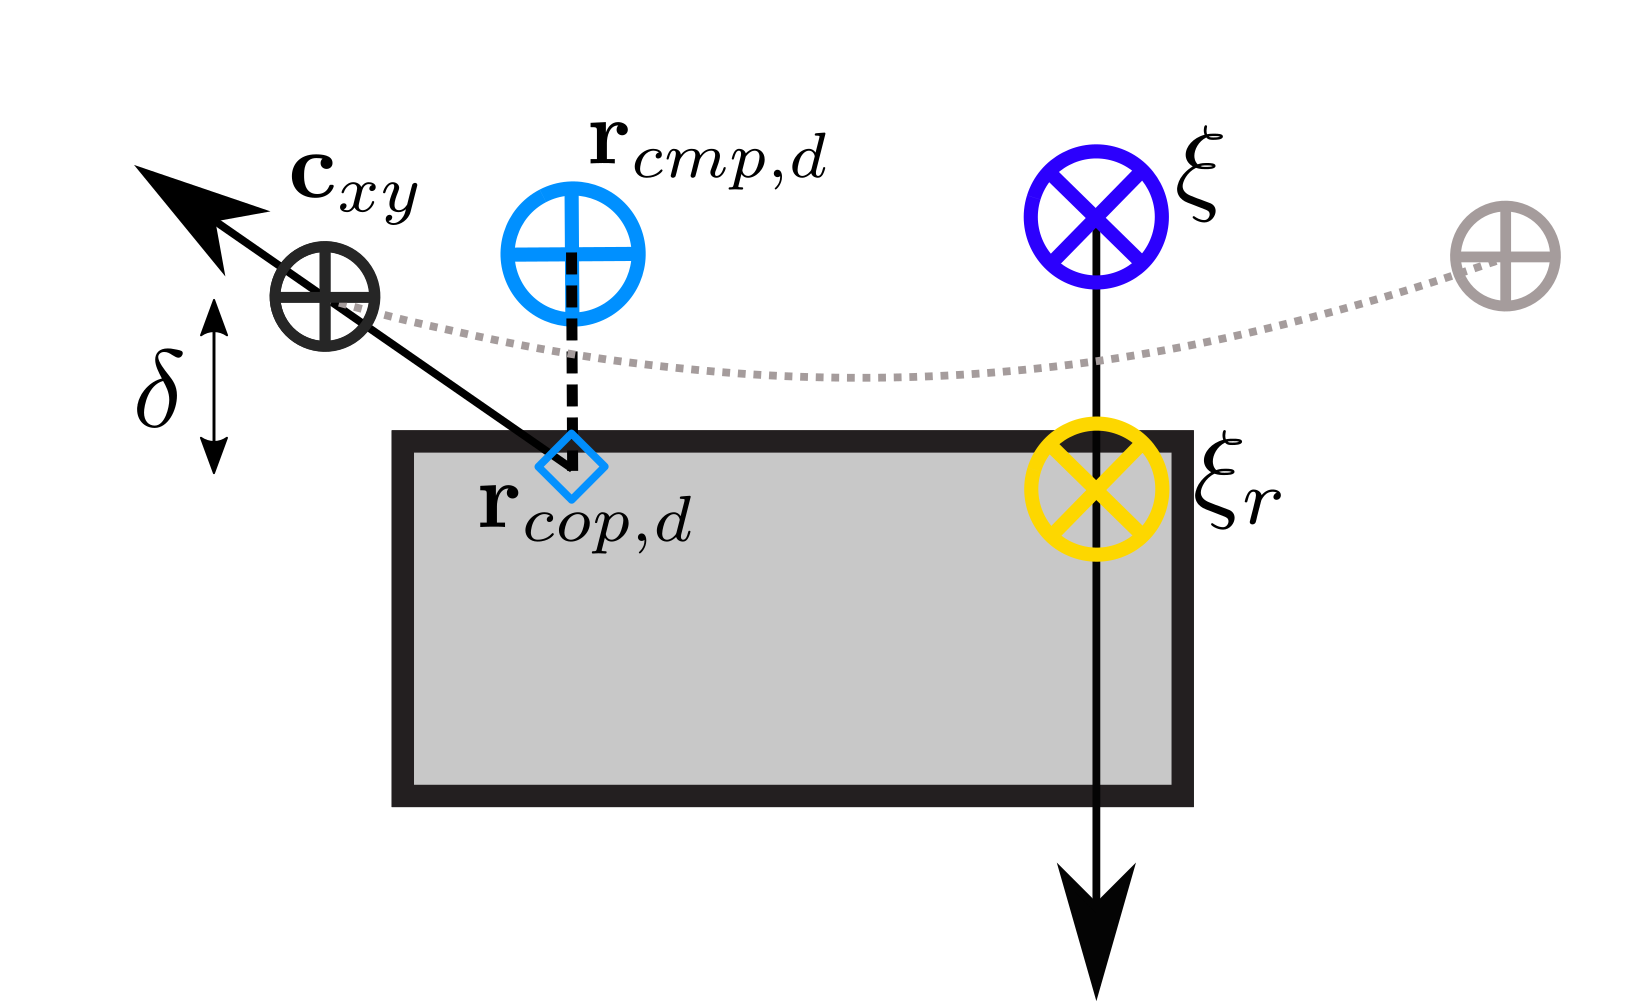
\includegraphics[width=.8\linewidth]{STYLESTUFF/ICPplanStartSSPhiVizRightError.png}
    \caption{}
     \label{fig:phiVizf}
  \end{subfigure}
  \caption{Vizualizations of the error alignment angle for the configuration at start of \ac{SS}, with \ac{ICP} errors: (a) negative in sagital plane, (b) positive in sagital plane, (c) where the error alignment angle is $0$ and (d) where the error alignment angle is orthogonal to the \ac{ICP} error. }
  \label{fig:phiViz}
\end{figure}

%QPbased - Only remarks, not in method?
\subsection{Quadratic Program Based}
One method: use lower weight on vertical momentum rate. To avoid singularity, a feedback based on a virtual spring, priviliged joint accelerations can be projected in the null-space. 

\begin{table}[ht]
\caption{Major affected tasks by $\mathbf{\dot{l}}_{xy,d}$ in whole-body QP, if \ac{CoP} is saturated.} % title of Table
\centering % used for centering table
\begin{tabular}{c c c } % centered columns (4 columns)
\hline\hline %inserts double horizontal lines
Affected Desired & Constraint/Consideration & Centroidal Momentum Rate \\
%heading
\hline % inserts single horizontal line
 $z_d$ & Leg singularity & Linear\\
 $\boldsymbol{\phi}_{body,d}$ & Upper body pose & Angular\\
 $\mathbf{r}_{foot,d}$ &  Touchdown time & Angular\\
%[1ex] % [1ex] adds vertical space
\hline %inserts single line
\end{tabular}
\label{tab:eatqp} % is used to refer this table in the text
\end{table}
